\begin{figure}[!ht]
	\centering
	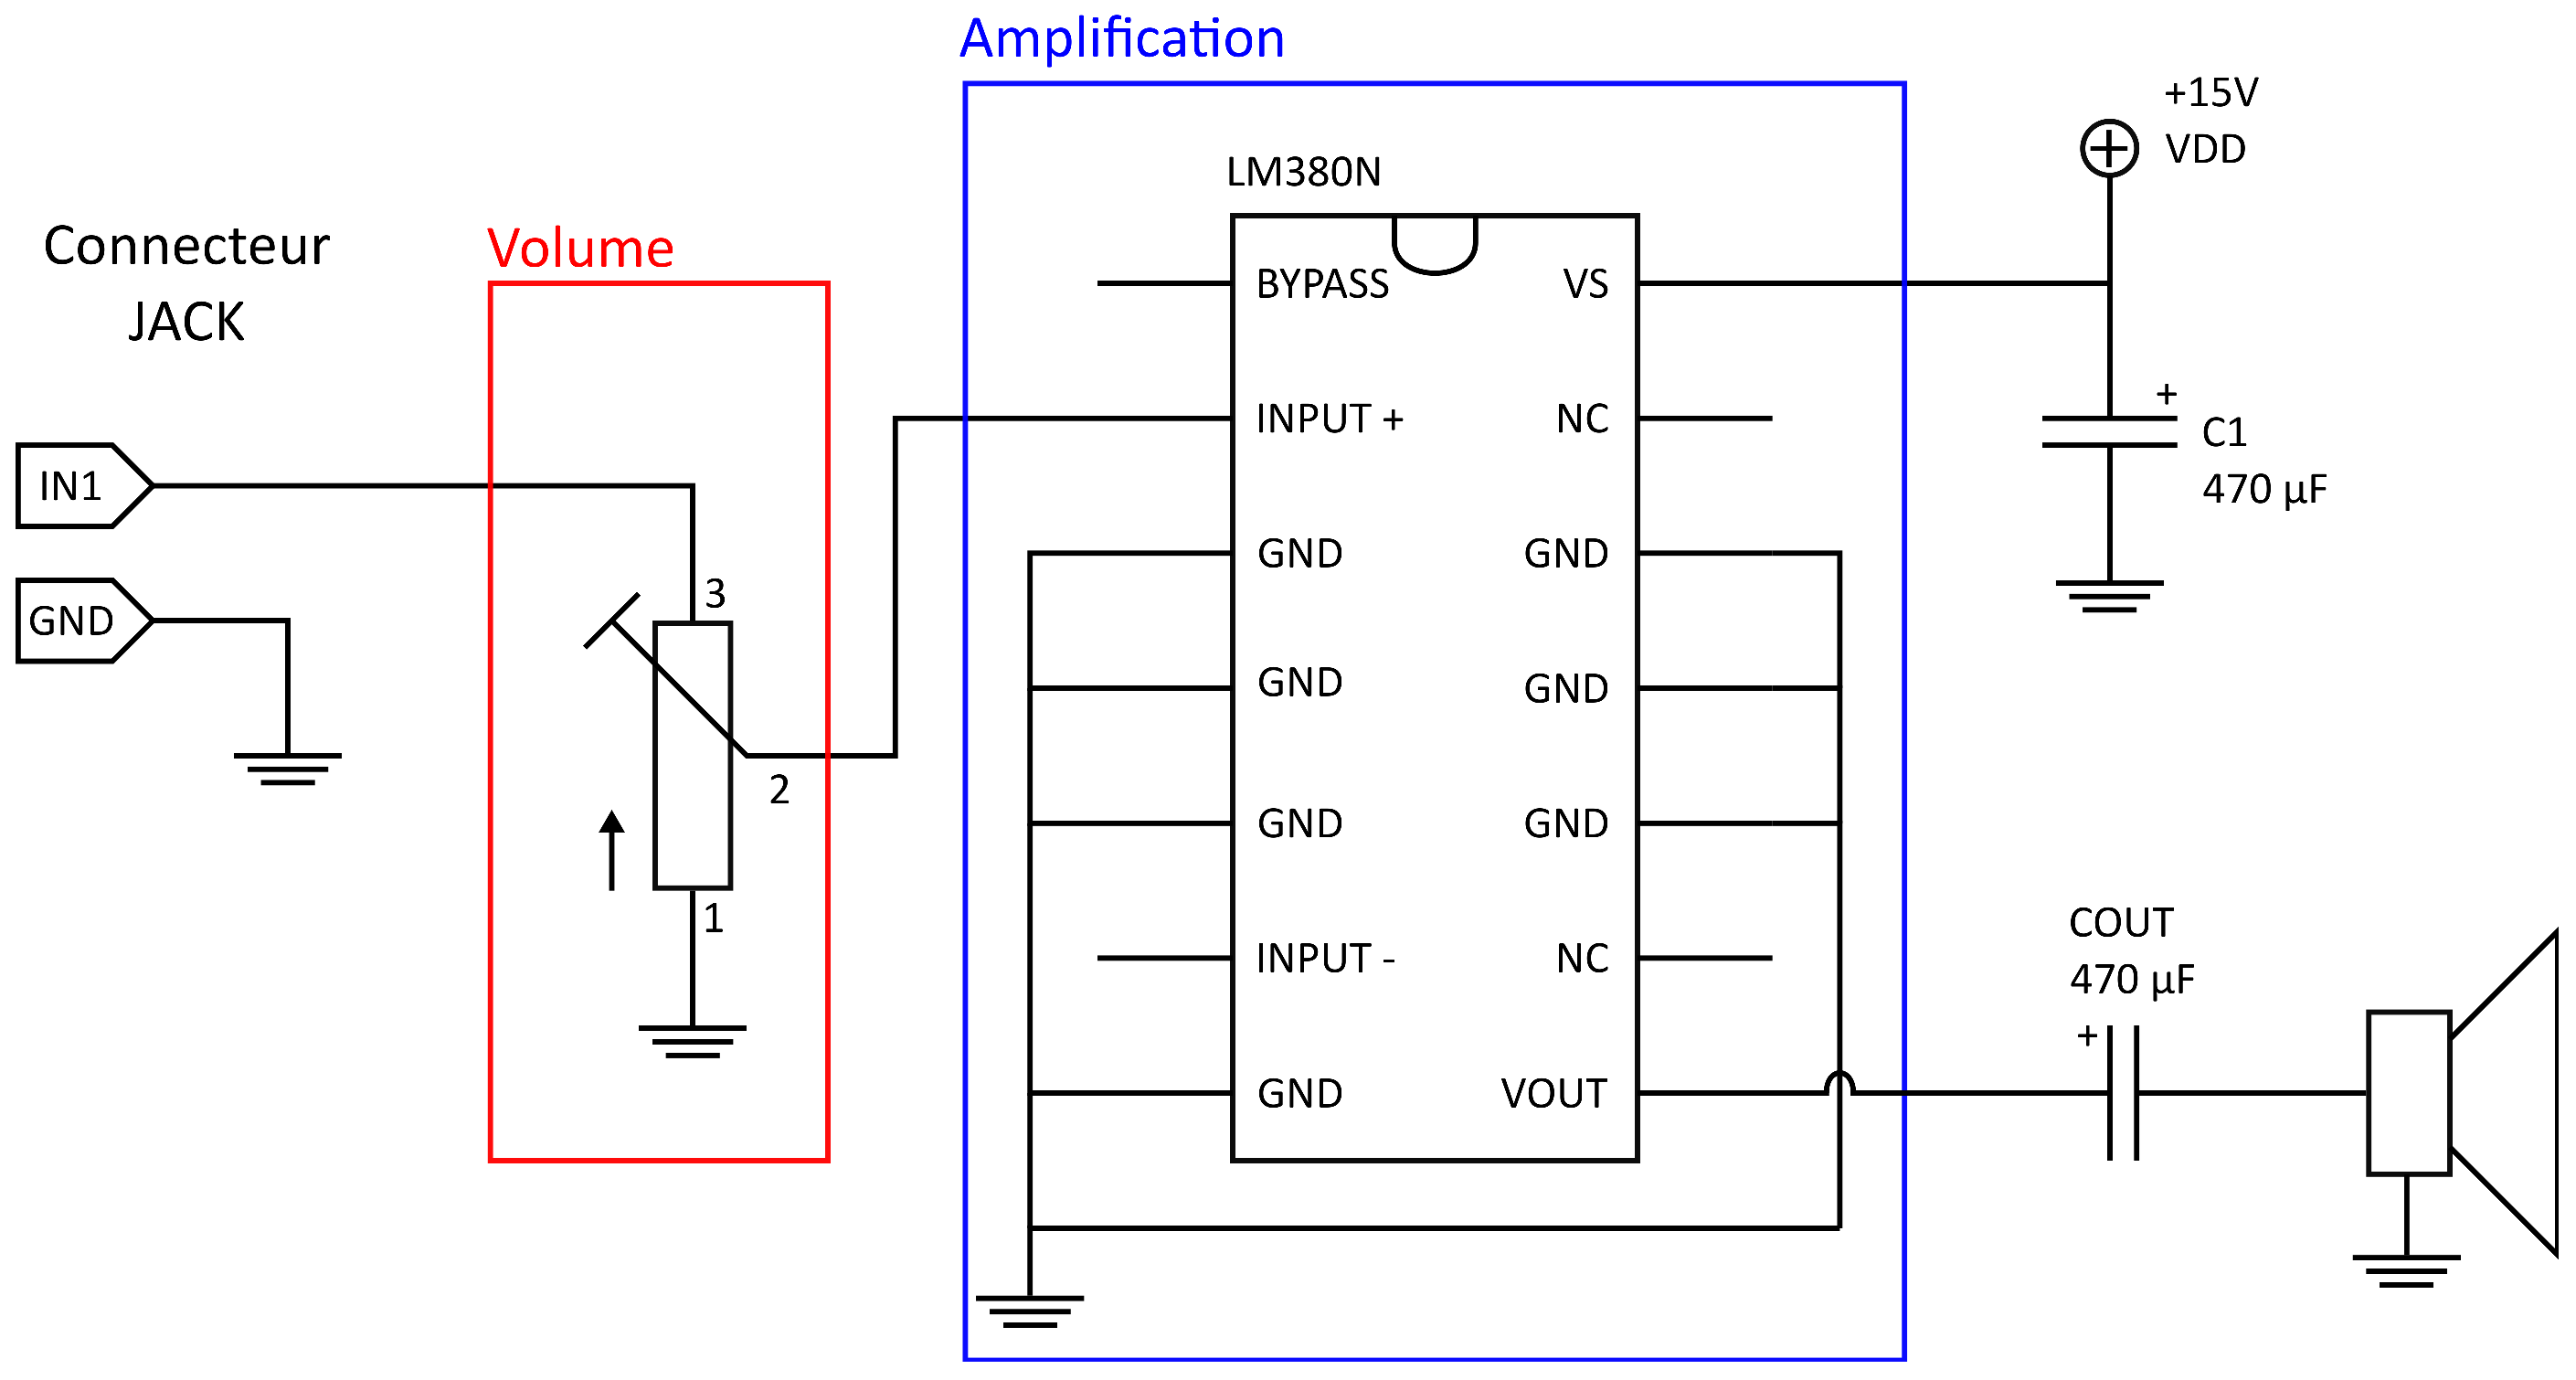
\includegraphics[width=.7\textwidth]{figures/schematics.eps}
	\caption{Schématique du circuit}
	\label{fig:schematics}
\end{figure}

Le schématique du circuit est présenté à la Figure \ref{fig:schematics}. Sur la gauche, le connecteur Jack amène une entrée IN1 et une référence de masse (notée GND) au circuit. L'entrée IN1 passe ensuite dans un diviseur résistif, implémenté sur base d'un potentiomètre, qui permet de modifier son amplitude. Cela permet donc de contrôler le volume du signal audio. Enfin, le signal sortant du diviseur résistif est amplifié dans un amplificateur audio LM380N, avant d'être envoyé vers le buzzer piézoélectrique ou le baffle.